\chapter{并发}\label{ch19}

\emph{In the long run it is not advisable to write large concurrent programs in machine-oriented languages that permit unrestricted use of store locations and their addresses. There is just no way we will be able to make such programs reliable (even with the help of complicated hardware mechanisms).}

\begin{flushright}
    ——Per Brinch Hansen (1977)
\end{flushright}

\emph{Patterns for communication are patterns for parallelism.}

\begin{flushright}
    ——Whit Morriss
\end{flushright}

如果你在职业生涯之中对并发的态度发生了改变,那你并不孤单,这是一种很常见的情况。

一开始的时候,编写并发代码是轻松并且愉快的。那些工具——线程,锁,队列等等——很容易上手和使用。虽然说实话也有很多的陷阱,但幸运的是你知道它们都是什么,所以你可以小心地不犯错误。

但有时,你不得不调试一些别人的多线程代码,然后你被迫得出结论:\emph{有些人}确实不应该使用这些工具。

然后有时你必须调试你自己的多线程代码。

经验会让你怀疑所有的多线程代码是否健康。少数的文章解释了为什么一些明显正确的多线程惯用写法完全不能工作,它们也许会有帮助。(它与“内存模型”有关。)但你最终会找到一种并发的方式,并且你觉得你能实际使用它且不会一直出错。你可能会把很多东西都塞进这种方法中,并且(如果你\emph{真的}很棒)你学会了对添加的复杂性说“不”。

当然,有很多种这样的方法。系统级程序员经常使用的方法包括下面这些:
\begin{enumerate}
    \item 一个只处理单个任务的\emph{后台线程(background thread)},周期性地唤醒它执行任务。
    \item 通用的\emph{线程池(worker pool)},通过\emph{任务队列(task queue)}和客户端交互。
    \item \emph{流水线(pipeline)},数据从一个线程流向下一个,每个线程都做一些工作。
    \item \emph{数据并行(data parallelism)},假设整个计算机主要在做很大型的计算,因此将数据分成\emph{n}片然后在\emph{n}个线程上运行,以让机器的\emph{n}个核心一起工作。
    \item \emph{同步对象之海(a sea of synchronized objects)},多个线程都有同一个数据的访问权限,使用基于底层原语例如mutex的ad hoc \emph{锁(lock)}方案来避免竞争。(Java内建了对这种模型的支持,这种模型在20世纪90年代和21世纪初非常流行。)
    \item \emph{原子整数操作(atomic integer operation)}允许多个核通过一个机器字大小的字段传递信息来通信。(这比其他方式更难正确实现,除非交换的数据实际上只是整数值。在实践中,它通常是指针。)
\end{enumerate}

随着时间的推移,你可能可以使用多种方式并安全地组合在一起。这时,你就是大师。如果没有其他人被允许修改系统,那么一切都会正常运作。正确使用线程的程序充满了不成文的规则。

Rust提供了一种更好的方式来使用并发,它并不强迫所有的程序使用单一的风格(这对系统级程序员来说并不是解决方案),而是安全地支持多种风格。不成文的规则现在被写下来了——就在代码中——并且被编译器强迫遵循。

你可能听说过Rust可以让你编写安全、快速、并发的程序。本章我们将向你展示如何做到这些。我们将介绍三种使用Rust线程的方式:
\begin{enumerate}
    \item fork-join并行
    \item channel
    \item 共享可变状态
\end{enumerate}

在此过程中,你将用到目前为止学过的所有Rust语言的知识。Rust关心的引用、可变性、生命周期在单线程程序中也很有价值,但只有在并发程序中这些规则真正的重要性才会显现出来。它们可以扩展你的工具箱,快速正确地破解多种风格的多线程代码——skepticism,没有cynicism,没有fear。

\section{fork-join并行}
多线程最简单的使用场景是我们有几个想同时执行的完全独立的任务。例如,假设我们要对非常多的文档进行自然语言处理。我们可以编写一个循环:
\begin{minted}{Rust}
    fn process_files(filenames: Vec<String>) -> io::Result<()> {
        for document in filenames {
            let text = load(&document)?;    // 读取源文件
            let results = process(text);    // 计算数据
            save(&document, results)?;      // 写入到输出文件
        }
        Ok(())
    }
\end{minted}

这个程序的运行情况如\autoref{f19-1}所示:

\begin{figure}[htbp]
    \centering
    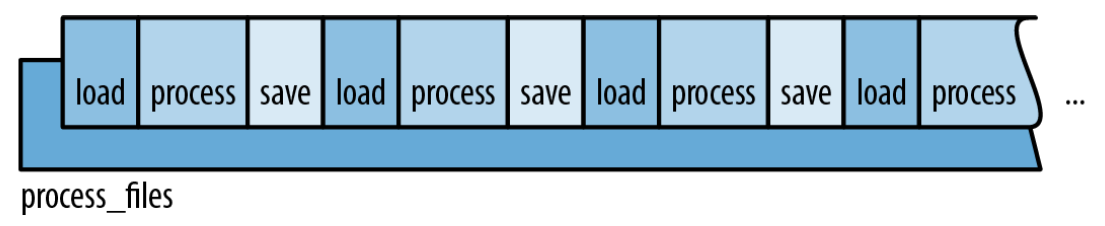
\includegraphics[width=0.9\textwidth]{../img/f19-1.png}
    \caption{单线程的\texttt{process\_files()}执行过程}
    \label{f19-1}
\end{figure}

因为每一个文档都是被单独处理,所以可以很容易的把所有文档分成几块、每一块在单独的线程中进行处理来加快速度,如\autoref{f19-2}所示。

\begin{figure}[htbp]
    \centering
    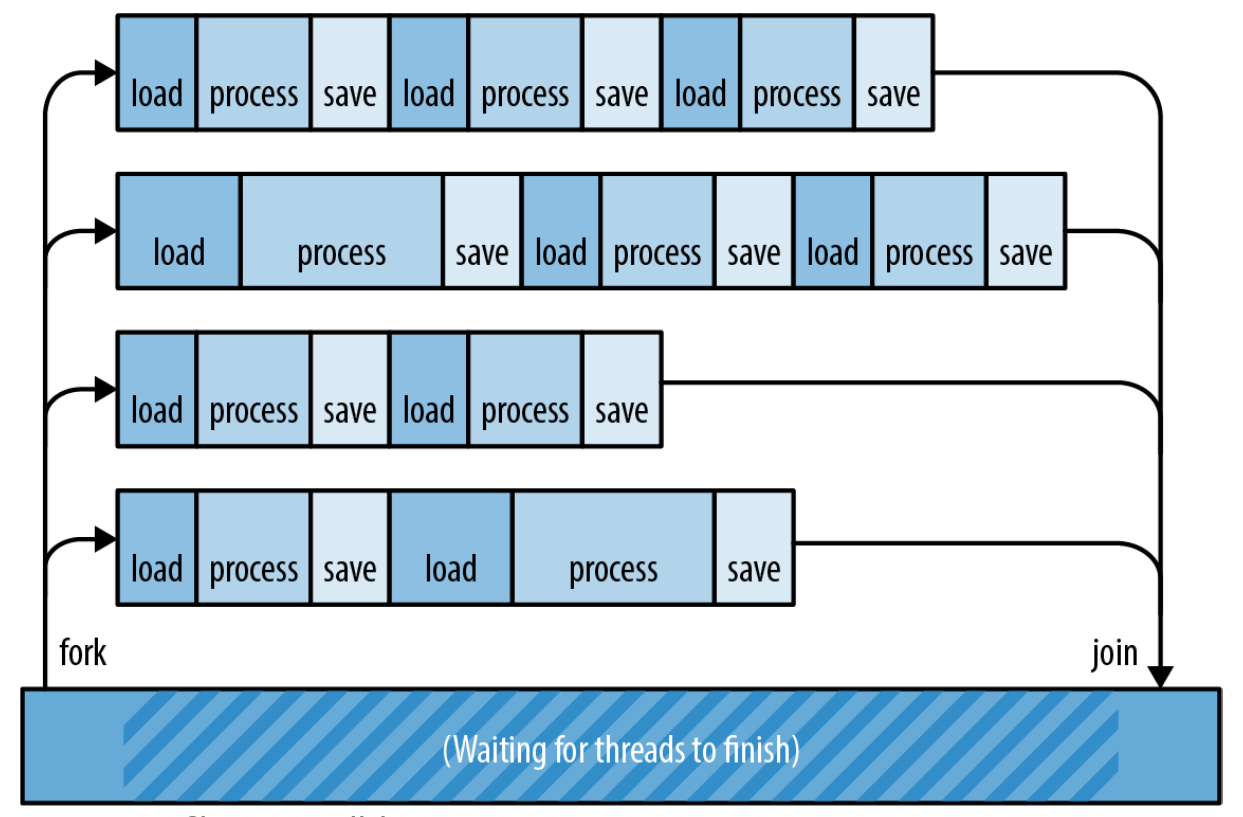
\includegraphics[width=0.8\textwidth]{../img/f19-2.png}
    \caption{使用fork-join方法的多线程文件处理}
    \label{f19-2}
\end{figure}

这个模式被称为\emph{fork-join并行}。\emph{fork}是启动一个新的线程,\emph{join}一个线程是等待它结束。我们已经看到过这个技术了:我们在\hyperref[ch02]{第2章}中使用了它来加速曼德勃罗集程序。

fork-join并行的优势主要在以下几个方面:
\begin{enumerate}
    \item 它太简单了。fork-join非常容易实现,并且Rust能帮你很轻松地保证它正确。
    \item 它避免了瓶颈。fork-join中没有共享资源的加锁。每个线程唯一要等待的时间就是最后要等待另一个线程结束。同时,每一个线程都可以自由地运行。这有助于保证很低的任务切换开销。
    \item 性能也非常直观。在最好的情况下,通过启动4个线程,我们可以用$\frac{1}{4}$的时间完成任务。\autoref{f19-2}展示了为什么我们不应该期待这种理想的加速:我们可能不能均匀地把工作分布到所有的线程上。另一个要注意的原因是一些fork-join程序在所有的线程结束之后还要花费一些时间\emph{组合(combine)}所有线程计算出的结果。即,完全分割任务可能要花费一些额外的工作。如果不考虑这两个原因,一个任务可以分割为独立单元的CPU密集的程序可以期待显著的性能提升。
    \item 很容易推断程序的正确性。只要每个线程真的被隔离,那么一个fork-join程序是\emph{确定性的(deterministic)},例如曼德勃罗集程序中的计算线程。程序总是会产生相同的结果,和线程速度的变化无关。它是一种没有竞争条件的并发模型。
\end{enumerate}

fork-join的主要缺点是它需要无关的任务单元。本章稍后我们会考虑一些不能分割的这么清晰的问题。

现在,让我们继续看自然语言处理的例子。我们将展示一些将fork-join模式应用于\texttt{process\_files}函数的方式。

\subsection{\texttt{spawn}和\texttt{join}}\label{spawn}
函数\texttt{std::thread::spawn}启动一个新线程:
\begin{minted}{Rust}
    use std::thread;

    thread::spawn(|| {
        println!("hello from a child thread");
    });
\end{minted}

它接受一个参数:一个\texttt{FnOnce}闭包或者函数。Rust启动一个新的线程来运行这个闭包或者函数。新的线程是一个真实的操作系统线程,有自己的栈,就类似于C++、C\#、Java中的线程。

这里有一个例子,使用\texttt{spawn}来实现之前的\texttt{process\_files}函数的一个并行版本:
\begin{minted}{Rust}
    use std::{thread, io};

    fn process_files_in_parallel(filenames: Vec<String>) -> io::Result<()> {
        // 把工作分成几块。
        const NTHREADS: usize = 8;
        let worklists = split_vec_into_chunks(filenames, NTHREADS);

        // Fork:创建一个新线程来处理每一个块。
        let mut thread_handles = vec![];
        for worklist in worklists {
            thread_handles.push(
                thread::spawn(move || process_files(worklist))
            );
        }

        // Join:等待所有线程结束。
        for handle in thread_handles {
            handle.join().unwrap()?;
        }

        Ok(())
    }
\end{minted}

让我们逐行分析这个函数。
\begin{minted}{Rust}
    fn process_files_in_parallel(filenames: Vec<String>) -> io::Result<()> {
\end{minted}

我们的新函数和原本的\texttt{process\_files}有完全相同的类型签名,这让它可以更轻松地替换原来的函数。

\begin{minted}{Rust}
        // 把工作分成几块。
        const NTHREADS: usize = 8;
        let worklists = split_vec_into_chunks(filenames, NTHREADS);
\end{minted}

我们使用了一个工具函数\texttt{split\_vec\_into\_chunks}来分割任务,不过这里没有显示。分割的结果\texttt{worklists}是一个vector的vector。它包含原本的vector \texttt{filenames}均匀分配的8个部分。

\begin{minted}{Rust}
        // Fork:创建一个新线程来处理每一个块。
        let mut thread_handles = vec![];
        for worklist in worklists {
            thread_handles.push(
                thread::spawn(move || process_files(worklist))
            );
        }
\end{minted}

我们为每一个\texttt{worklist}启动了一个线程。\texttt{spawn()}返回一个称为\texttt{JoinHandle}的值,我们之后会使用它。现在,我们只是将所有的\texttt{JoinHandle}放进一个vector里。

注意我们如何把文件名的列表传进工作线程里:
\begin{enumerate}
    \item \texttt{worklist}在父线程的\texttt{for}循环中定义和初始化。
    \item 一旦\texttt{move}闭包创建完成,\texttt{worklist}就会被移动进闭包里
    \item 然后\texttt{spawn}把闭包(包括\texttt{worklist})移动进新的子线程。
\end{enumerate}

这些移动操作开销很小。正如我们在\hyperref[ch04]{第4章}中讨论的\texttt{Vec<String>}的移动一样,\texttt{String}并不会被拷贝。事实上,没有任何东西被分配或者释放。唯一被移动的数据是\texttt{Vec}自己:三个机器字。

你创建的大多数线程都同时需要代码和数据才能运行。Rust闭包可以便捷地包含了你需要的代码和数据。。

继续:
\begin{minted}{Rust}
        // Join:等待所有线程结束。
        for handle in thread_handles {
            handle.join().unwrap()?;
        }
\end{minted}

我们使用了之前收集的\texttt{JoinHandle}的\texttt{.join()}方法来等待8个线程全部结束。为了保证正确性,join线程通常是必须的,因为一旦\texttt{main}返回Rust程序就会退出,即使其他的线程仍然在运行。析构器不会被调用,额外的线程被简单地杀死。如果这不是你想要的,确保在\texttt{main}返回之前join所有你关心的线程。

如果这个循环结束了,那么意味着8个子线程都已经成功结束。我们的函数返回一个\texttt{Ok(())}并结束:
\begin{minted}{Rust}
        Ok(())
    }
\end{minted}

\subsection{跨线程的错误处理}
我们的例子中用来join子线程的代码比看起来更加有趣,因为还要考虑错误处理。让我们回顾这一行代码:
\begin{minted}{Rust}
    handle.join().unwrap()?;
\end{minted}

\texttt{.join()}方法给我们带来了两个问题。

首先,\texttt{handle.join()}返回一个\texttt{std::thread::Result},\emph{如果子线程panic}那么它的值将是一个错误。这使得Rust中的线程比C++中更健壮。在C++中,一个越界的数组访问是未定义行为,并且没有办法保护系统中的其他部分不受其影响。在Rust中,\hyperref[unwind]{panic是安全的并且以线程为单位}。线程之间的边界充当panic时的防火墙;panic并不会自动从一个线程传播到依赖它的线程。一个线程中的panic在其他线程中作为一个值为错误的\texttt{Result}汇报。整个程序可以不受其影响。

在我们的程序中,我们没有尝试任何panic的处理。我们简单地对返回的\texttt{Result}调用\texttt{.unwrap()},假定它它是一个\texttt{Ok}的结果而不是\texttt{Err}的结果。如果一个子线程\emph{确实}panic了,那么这个断言会失败,因此父线程也会panic。我们显式地把子线程的panic传播到父线程。

其次,\texttt{handle.join()}会把子线程返回的值传递给父线程。我们传递给\texttt{spawn}的闭包的返回类型是\texttt{io::Result<()>},因为\texttt{process\_files}返回这个类型。这个返回值不会被丢弃,当子线程结束时,它的返回值会被保存,\texttt{JoinHandle::join()}会把值传递给父线程。

这个程序中\texttt{handle.join()}返回的完整类型是\texttt{std::thread::Result<std::io::Result<()>>}。\texttt{thread::Result}是\texttt{spawn/join} API的一部分;\texttt{io::Result}是我们程序的一部分。

在我们的例子中,解包了\texttt{thread::Result}之后,我们对\texttt{io::Result}使用了\texttt{?}运算符,显式地把子线程的I/O错误传播给父线程。

整个过程看起来可能很复杂,但这其实也只是一行代码的功能。将它与其它语言比较:Java和C\#中的默认行为是将子线程的异常转储到终端,然后忽略。在C++中,默认行为是终止进程。在Rust中,错误是\texttt{Result}值(数据)而不是异常(控制流)。它们像其他任何值一样在线程之间传递。每一次你使用底层线程的API时,你都必须小心地编写错误处理代码,但考虑到\emph{你必须编写它们},所以Rust在这一点上做得很好。

\subsection{跨线程共享不可变数据}
假设我们正在进行的分析需要一个非常大的由英文单词和短语组成的数据库:
\begin{minted}{Rust}
    // 之前
    fn process_files(filenames: Vec<String>)

    // 之后
    fn process_files_in_parallel(filenames: Vec<String>, glossary: &GigabyteMap)
\end{minted}

\texttt{glossary}可能很大,所以我们通过引用传递它。我们应该如何更新\texttt{process\_files\_in\_parallel}来在多个工作线程间传递词汇表呢?

显而易见的修改方法并不能工作:
\begin{minted}{Rust}
    fn process_files_in_parallel(filenames: Vec<String>,
                                 glossary: &GigabyteMap)
        -> io::Result<()>
    {
        ...
        for worklist in worklists {
            thread_handles.push(
                spawn(move || process_files(worklist, glossary))    // 错误
            );
        }
        ...
    }
\end{minted}

我们只是简单地给函数添加了一个\texttt{glossary}参数并把它传递给\texttt{process\_files}。Rust会报错:
\begin{minted}{text}
    error[E0621]: explicit lifetime required in the type of `glossary`
      --> src/lib.rs:75:17
       |
    61 |     glossary: &GigabyteMap)
       |               ------------ help: add explicit lifetime `'static` to the 
                                    type of `glossary`: `&'static BTreeMap<String,
                                    String>`
    ...
    75 |                 spawn(move || process_files(worklist, glossary))
       |                 ^^^^^ lifetime `'static` required
\end{minted}

Rust在抱怨我们传递给\texttt{spawn}的闭包的生命周期,编译器给出的“有帮助的”信息实际上也没有一点帮助。

\texttt{spawn}启动独立的线程。Rust没有办法直到子线程会运行多长时间,因此它假设最坏的情况:它假设子线程会一直保持运行,然而在父线程结束之后父线程里的所有值都会消失。显然,如果子线程要持续很长时间,那么它运行所需要的闭包也应该持续这么长时间。但这个闭包有一个有界的生命周期:它依赖于引用\texttt{glossary},但引用并不会一直有效。

注意Rust拒绝这段代码是正确的!按照我们编写这个函数的方式,\emph{有可能}一个线程遇到I/O错误,导致\texttt{process\_files\_in\_parallel}在其他线程结束之前结束。子线程可能会在主线程释放\texttt{glossary}之后仍然尝试使用它。这会导致未定义行为。Rust不允许出现这种情况。

看起来\texttt{spawn}太过开放以至于不能支持跨线程共享引用。事实上,我们已经在“\nameref{StealClosure}”中见到过一个类似于这样的例子。那一次我们的解决方案是使用\texttt{move}闭包把数据的所有权移动到新线程里。但那种方法在这里不能生效,因为我们有很多线程需要使用相同的数据。一个安全的替代方案是为每一个线程\texttt{clone}一份词汇表,但因为它很庞大,我们希望避免这些开销。幸运的是,标准库提供了另一种方案:自动引用计数。

我们在“\nameref{rc}”中介绍过\texttt{Arc}。现在正是使用它的时候:
\begin{minted}{Rust}
    use std::sync::Arc;

    fn process_files_in_parallel(filenames: Vec<String>,
                                 glossary: Arc<GigabyteMap>)
        -> io::Result<()>
    {
        ...
        for worklist in worklists {
            // 这里的.clone()调用只会克隆Arc并递增引用计数。
            // 它并不会克隆GigabyteMap。
            let glossary_for_child = glossary.clone();
            thread_handles.push(
                spawn(move || process_files(worklist, &glossary_for_child))
            );
        }
        ...
    }
\end{minted}

我们改变了\texttt{glossary}的类型:为了进行并行分析,调用者必须传递一个\texttt{Arc<GigabyteMap>},它是使用\texttt{Arc::new(giga\_map)}创建的一个指向堆上的\texttt{GigabyteMap}的智能指针。

当我们调用\texttt{glossary.clone()}时,我们是在创建\texttt{Arc}智能指针的一个拷贝,而不是整个\texttt{GigabyteMap}的拷贝。它只会递增一个引用计数。

修改之后,程序就可以编译运行了,因为它不再依赖引用的生命周期。只要有\emph{任何}线程还持有一个\texttt{Arc<GigabyteMap>},它就会保持词汇表仍然存在,即使父线程提前退出。也不会有任何数据竞争,因为\texttt{Arc}里的数据是不可变的。

\subsection{Rayon}

标准库的\texttt{spawn}函数是一个重要的原语,但它并不是专为fork-join并行设计的。还有基于它们构建的更好的fork-join API。例如,“\nameref{ch02}”中我们使用了Crossbeam库把一些任务分割给8个进程。Crossbeam的\emph{scoped thread(作用域线程)}非常自然地支持fork-join并行。

Niko Matsakis和Josh Stone编写的Rayon库是另外一个例子。它提供两种并发运行任务的方法:
\begin{minted}{Rust}
    use rayon::prelude::*;

    // 并行做2件事
    let (v1, v2) = rayon::join(fn1, fn2);

    // 并行做N件事
    giant_vector.par_iter().for_each(|value| {
        do_thing_with_value(vaue);
    });
\end{minted}

\texttt{rayon::join(fn1, fn2)}同时调用两个函数并返回两个结果。\texttt{.par\_iter()}方法创建一个\texttt{ParallelIterator},它有\texttt{map}、\texttt{filter}以及其它的方法,非常像Rust中的\texttt{Iterator}。在这两种情况下,Rayon都会尽可能使用它自己的工作线程池来处理任务。你只需要告诉Rayon什么样的任务\emph{可以}并行完成;Rayon负责管理线程并尽可能好地分发任务。

\autoref{f19-3}展示了有关调用\texttt{giant\_vector().par\_iter().for\_each(...)}的两种思考方式:(a) Rayon为vector中的每个元素创建一个线程。(b) Rayon在幕后维护等同于CPU核数个工作线程,每个工作线程运行在每个CPU核上,这样会更加高效。工作线程池被程序的所有线程共享,当同时有上千个任务到达时,Rayon会划分任务。

\begin{figure}[htbp]
    \centering
    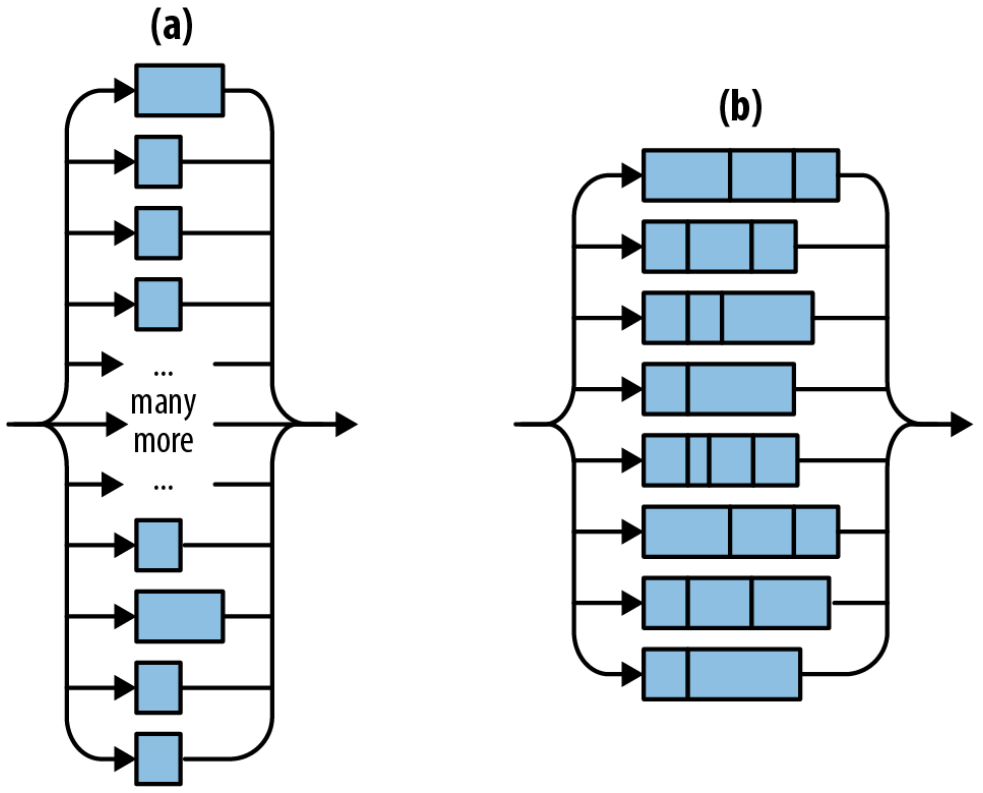
\includegraphics[width=0.9\textwidth]{../img/f19-3.png}
    \caption{理论和实践中的Rayon}
    \label{f19-3}
\end{figure}

这里有一个使用Rayon的\texttt{process\_files\_in\_parallel}的版本,并且它要运行的\texttt{process\_file}函数,不再需要\texttt{Vec<String>},而是需要\texttt{\&str}:
\begin{minted}{Rust}
    use rayon::prelude::*;

    fn process_files_in_parallel(filenames: Vec<String>, glossary: &GigabyteMap)
        -> io::Result<()>
    {
        filenames.par_iter()
            .map(|filename| process_file(filename, glossary))
            .reduce_with(|r1, r2| {
                if r1.is_err() { r1 } else { r2 }
            })
            .unwrap_or(Ok(()))
    }
\end{minted}

这段代码比使用\texttt{std::thread::spawn}的版本更加简短,也更加容易理解。让我们逐行分析它:
\begin{enumerate}
    \item 首先,我们使用了\texttt{filenames.par\_iter()}来创建一个并行迭代器。
    \item 我们使用\texttt{.map()}来对每一个文件名调用\texttt{process\_file}。这会返回一个产生\texttt{io::Result<()>}值的序列的\texttt{ParallelIterator}。
    \item 我们使用\texttt{.reduce\_with()}来组合结果。这里我们保留了第一个错误并丢弃剩余的内容。如果我们想累计所有的错误,或者打印它们,我们可以在这里完成。
    \item 当你向\texttt{.map()}传递一个在成功时会返回有用值的闭包时,\texttt{.reduce\_with()}方法也非常方便。你可以向\texttt{.reduce\_with()}传递一个知道如何组合两个成功结果的闭包。
    \item \texttt{reduce\_with}返回一个\texttt{Option},只有当\texttt{filenames}为空时它是\texttt{None}。我们使用了\texttt{Option}的\texttt{.unwrap\_or()}方法以在这种情况下产生一个\texttt{Ok(())}。
\end{enumerate}

在幕后,Rayon会使用一种叫做\emph{work-stealing}的技术动态地实现多个线程的负载均衡。通常保持所有CPU核心忙碌比“\nameref{spawn}”中的事先手动划分任务效果会更好。

作为奖励,Rayon支持在线程之间共享引用。所有幕后的并行处理都保证在\texttt{reduce\_with}返回之前结束。这解释了为什么我们可以向\texttt{process\_file}传递\texttt{glossary},即使这个闭包将会在多个线程间调用。

(顺便说一下,我们使用\texttt{map}和\texttt{reduce}方法并不是巧合。被Google和Apache Hadoop推广的MapReduce编程模型和fork-join方法有很多相同之处。它可以被看做处理分布式数据的fork-join方法。

\subsection{回顾曼德勃罗集}

\section{通道}

\subsection{发送值}

\subsection{接收值}

\subsection{运行管道}

\subsection{通道的特性和性能}

\subsection{线程安全:\texttt{Send}和\texttt{Sync}}\label{threadsafe}

\section{共享可变状态}

\subsection{自旋锁是什么?}

\subsection{Mutex<T>}\label{mutex}

\subsection{mut和Mutex}

\subsection{为什么有时自旋锁不是好的方案}

\subsection{死锁}

\subsection{中毒的自旋锁}

\subsection{使用自旋锁的多消费者channel}

\subsection{读写锁(RwLock<T>)}

\subsection{条件变量(Condvar)}

\subsection{原子量}\label{atomic}

\subsection{全局变量}\label{globalvar}